\newpage
\section{Control Region}
\label{sec:control_region}
\ifboth

%------------------------------------------------------------------
\subsection{Same-sign di-muon control region}
\label{sec:ss_control_region}
%------------------------------------------------------------------



The signal region of this analysis targets opposite-sign di-muon pairs ($\mu^+\mu^-$), where BSM processes such as $T' \rightarrow \mu^+\mu^- + X$ would produce a localized excess in the $m_{\mu\mu}$ spectrum.
To validate the CATHODE anomaly detection methodology in a data-driven setting free of signal contamination, a same-sign di-muon control region is constructed by selecting pairs of muons carrying identical charge ($\mu^+\mu^+$ or $\mu^-\mu^-$).
 
Our search targets resonances decaying to opposite sign muon pairs, so the same-sign sample is free of such contributions.
SM backgrounds arise mostly from non-prompt and misidentified muons, with no reason to expect peaking structures in the invariant mass distribution.
This makes the same-sign region an ideal ideal as a control region.
Running our procedure on a smooth, signal-free control region allows verification that the method does not generate spurious excesses in the absence of true new physics, and any sculpting artifacts introduced by the anomaly detection pipeline can be identified before unbinding.

% \TODO[Add quantitative signal suppression plots confirming the same-sign/opposite-sign significance ratio is $\lesssim 10\%$ for the benchmark signal models. The physics argument above (charge conservation) is strong, but a numerical demonstration using the signal MC samples would satisfy ARC review requirements.]
%Note: This should be satisfied by the Trigger analysis section Tamas is writing

% We do not use the 2025 dataset in this analysis as it currently lacks calibration. 
% \TODO[Formally justify the exclusion of 2025 scouting data from this analysis. State the reason explicitly here (e.g.\ trigger conditions, luminosity accounting, consistency with the primary analysis dataset) once this has been decided.]

%------------------------------------------------------------------
\subsection{Event Selection}
\label{sec:cr_event_selection}
%------------------------------------------------------------------

Events in the same-sign control region are required to satisfy the same selection criteria as the opposite-sign signal region (Sections~\ref{sec:event_quality}--\ref{sec:preselection}).

Events must pass the logical OR of the six dedicated double-muon L1 trigger seeds; the trigger seeds, their kinematic requirements, and their efficiencies are listed in Section~\ref{sec:trigger}.


%------------------------------------------------------------------
\subsection{Control Region Features}
\label{sec:cr_features}
%------------------------------------------------------------------

The same feature set described in Section~\ref{sec:feature_set} is used in the control region without modification: the Euclidean phase space coordinates, the scalar sum of non-signal jet $\pt$ ($H_T^\text{jets}$), and the missing transverse energy.

Using an identical feature set ensures that any sculpting artifacts observed in the control region are directly interpretable as potential issues in the signal region analysis.

The distributions of all input features in the same-sign control region are shown in Figs~\ref{fig:cr_dimuon_mass_MET}--\ref{fig:cr_Omega_z2_z3}, with data and simulated background (DY + QCD multijet + $t\bar{t}$) overlaid. Again we can observe the limited size of the QCD MC sample.

\begin{figure}[!h]
    \centering
    \includegraphics[width=0.45\linewidth]{Figures/6Control_Region_figures/Features/dimuon_mass_vr.pdf}
    \includegraphics[width=0.45\linewidth]{Figures/6Control_Region_figures/Features/dimuon_MET_vr.pdf}
    \caption{Di-muon invariant mass $m_{\mu\mu}$ (left) and missing transverse energy \MET (right) in the validation region.}
    \label{fig:cr_dimuon_mass_MET}
\end{figure}

\begin{figure}[!h]
    \centering
    \includegraphics[width=0.45\linewidth]{Figures/6Control_Region_figures/Features/dimuon_sum_jet_pt_vr.pdf}
    \includegraphics[width=0.45\linewidth]{Figures/6Control_Region_figures/Features/dimuon_multiplicity.pdf}
    \caption{Scalar sum of jet transverse momenta, $H_T^\text{jets}$ (left) and event multiplicity (right) in the validation region.}
    \label{fig:cr_sum_jet_pt_Multiplicity}
\end{figure}

\begin{figure}[!h]
    \centering
    \includegraphics[width=0.45\linewidth]{Figures/6Control_Region_figures/Features/dimuon_mass_coordinate_t1.pdf}
    \includegraphics[width=0.45\linewidth]{Figures/6Control_Region_figures/Features/dimuon_mass_coordinate_t2.pdf}
    \caption{Mass coordinates $\Omega_{m,1}$ (left) and $\Omega_{m,2}$ (right) in the validation region.}
    \label{fig:cr_mass_coordinate_1_2}
\end{figure}

\begin{figure}[!h]
    \centering
    \includegraphics[width=0.45\linewidth]{Figures/6Control_Region_figures/Features/dimuon_mass_coordinate_t3.pdf}
    \includegraphics[width=0.45\linewidth]{Figures/6Control_Region_figures/Features/dimuon_mass_coordinate_t4.pdf}
    \caption{Mass coordinates $\Omega_{m,3}$ (left) and $\Omega_{m,4}$ (right) in the validation region.}
    \label{fig:cr_mass_coordinate_3_4}
\end{figure}

\begin{figure}[!h]
    \centering
    \includegraphics[width=0.45\linewidth]{Figures/6Control_Region_figures/Features/dimuon_mass_coordinate_t5.pdf}
    \includegraphics[width=0.45\linewidth]{Figures/6Control_Region_figures/Features/dimuon_omega_x1_vr.pdf}
    \caption{Mass coordinate $\Omega_{m,5}$ (left) and stereographic coordinate $\Omega_{x,1}$ (right) in the validation region.}
    \label{fig:cr_mass_coordinate_5_Omega_x1}
\end{figure}

\begin{figure}[!h]
    \centering
    \includegraphics[width=0.45\linewidth]{Figures/6Control_Region_figures/Features/dimuon_omega_x2.pdf}
    \includegraphics[width=0.45\linewidth]{Figures/6Control_Region_figures/Features/dimuon_omega_x3.pdf}
    \caption{Stereographic coordinates $\Omega_{x,2}$ (left) and $\Omega_{x,3}$ (right) in the validation region.}
    \label{fig:cr_Omega_x2_x3}
\end{figure}

\begin{figure}[!h]
    \centering
    \includegraphics[width=0.45\linewidth]{Figures/6Control_Region_figures/Features/dimuon_omega_y1_vr.pdf}
    \includegraphics[width=0.45\linewidth]{Figures/6Control_Region_figures/Features/dimuon_omega_y2_vr.pdf}
    \caption{Stereographic coordinates $\Omega_{y,1}$ (left) and $\Omega_{y,2}$ (right) in the validation region.}
    \label{fig:cr_Omega_y1_y2}
\end{figure}

\begin{figure}[!h]
    \centering
    \includegraphics[width=0.45\linewidth]{Figures/6Control_Region_figures/Features/dimuon_omega_y3_vr.pdf}
    \includegraphics[width=0.45\linewidth]{Figures/6Control_Region_figures/Features/dimuon_omega_z1_vr.pdf}
    \caption{Stereographic coordinates $\Omega_{y,3}$ (left) and $\Omega_{z,1}$ (right) in the validation region.}
    \label{fig:cr_Omega_y3_z1}
\end{figure}

\begin{figure}[!h]
    \centering
    \includegraphics[width=0.45\linewidth]{Figures/6Control_Region_figures/Features/dimuon_omega_z2_vr.pdf}
    \includegraphics[width=0.45\linewidth]{Figures/6Control_Region_figures/Features/dimuon_omega_z3_vr.pdf}
    \caption{Stereographic coordinates $\Omega_{z,2}$ (left) and $\Omega_{z,3}$ (right) in the validation region.}
    \label{fig:cr_Omega_z2_z3}
\end{figure}

\newpage
%------------------------------------------------------------------
\subsection{Data/MC Comparison}
\label{sec:cr_mc}
%------------------------------------------------------------------

The purpose of the data/MC feature comparison --- validating the object reconstruction and event selection, and providing a cross-check that the background composition is understood before the CATHODE pipeline is applied --- is described for the signal region in Section~\ref{sec:feature_set}; the same comparison is shown here for the same-sign validation region.

The simulated background samples used for this comparison are the DY, $t\bar{t}$, QCD multijet, and $WW$ samples described in Section~\ref{sec:background_samples}, normalized to the data luminosity as described in Section~\ref{sec:luminosity}.
The validation-region distributions are those shown in Figs~\ref{fig:cr_dimuon_mass_MET}--\ref{fig:cr_Omega_z2_z3}; as in the signal region, the data are well described by the simulation apart from the tails, where the QCD MC sample size is limited.

\subsection{Feature correlation with mass}
\label{sec:cr_mc}

% A comparison of the same-sign data distributions with the simulated background prediction serves two purposes: it validates the object reconstruction and event selection for the scouting dataset, and it provides a cross-check that the background composition is well understood before the CATHODE pipeline is applied.

% The simulated background samples used for this comparison are the DY, $t\bar{t}$, QCD multijet, and $WW$ samples described in Section~\ref{sec:background_samples}, normalised to the data luminosity as described in Section~\ref{sec:luminosity}.


The requirement that the classifier input features be decorrelated from the di-muon mass, and the per-window test used to verify it, are described for the signal region in Section~\ref{sec:feature_mass_dependence}; the same test is repeated here for the same-sign validation region.
As in the signal region, the per-window feature distributions and their means are stable across the di-muon mass windows, showing no dependence on $m_{\mu^+\mu^-}$.
The representative stereographic coordinate $\Omega_{x,1}$ is shown in Fig.~\ref{fig:cr_mass_dep_omega_x1} for the non-zero entries (the values the flow models); the version including the structural zeros, and the remaining coordinates, show the same mass independence.

\begin{figure}[!h]
    \centering
    \includegraphics[width=0.9\linewidth]{Figures/6Control_Region_figures/Mass dependence/Zeroes Removed/x_stereo_0_mass_dep_x_stereo_0_nonzero_20260323_205142 copy.png}
    \caption{Mass dependence of the stereographic coordinate $\Omega_{x,1}$ in the same-sign validation region, restricted to events for which the coordinate is non-zero. Left: the normalized distribution of $\Omega_{x,1}$ in contiguous $5$\GeV\ di-muon mass windows, overlaid. Right: the per-window mean (markers, with the per-window standard deviation as an error bar) compared to the overall mean (dashed line). As in the signal region (Section~\ref{sec:feature_mass_dependence}), neither the shape nor the mean shows a systematic trend with $m_{\mu^+\mu^-}$.}
    \TODO{Add figure}
    \label{fig:cr_mass_dep_omega_x1}
\end{figure}


%------------------------------------------------------------------
\subsection{Pipeline validation in the same-sign data control region}
\label{sec:cr_pipeline_validation}
%------------------------------------------------------------------

The full CATHODE pipeline --- generative model training, synthetic background generation, weakly supervised classification, and bump hunt fit signal extraction --- is applied to the same-sign control region under the same conditions used in the signal region analysis.
The pipeline is run independently in each of the overlapping $5$\GeV\ wide mass windows that tile the search range, following the windowing described in Section~\ref{sec:mass_windows}.
A separate generative model and classifier are trained in every window, so that the anomaly selection is derived locally, exactly as in the signal region.
Within each window the validated bump-hunt fit of Section~\ref{sec:stat_procedure} is then performed at every mass hypothesis of the scan grid, with each hypothesis assigned to the single window whose centre is closest to it, so that no hypothesis is fit more than once.
The scan covers the full search range, comprising 119 mass hypotheses between 13.8 and 75.0\GeV\ distributed over 25 windows.

\newpage
%------------------------------------------------------------------
\subsubsection{Post-Fit Results Across Mass Windows}
\label{sec:cr_postfit_results}
%------------------------------------------------------------------

The pipeline is run over the full scan grid, yielding 119 signal-plus-background fits distributed over the 25 mass windows.
In each fit the background is described by the discrete-profiling envelope and the signal by the interpolated double Crystal Ball template at the corresponding mass hypothesis.

The background-only goodness of fit is summarized in Fig.~\ref{fig:cr_bkg_gof}.
Across the 119 fits the mean $p$-value is 0.50 and the median $\chi^2/\mathrm{ndof}$ is 0.99, and the distribution of $p$-values is consistent with uniform, as expected when the background model adequately describes the data.
No fit falls below $p=0.05$.
The set of functional forms is therefore able to describe the same-sign data across the full search range.

\begin{figure}[!h]
    \centering
    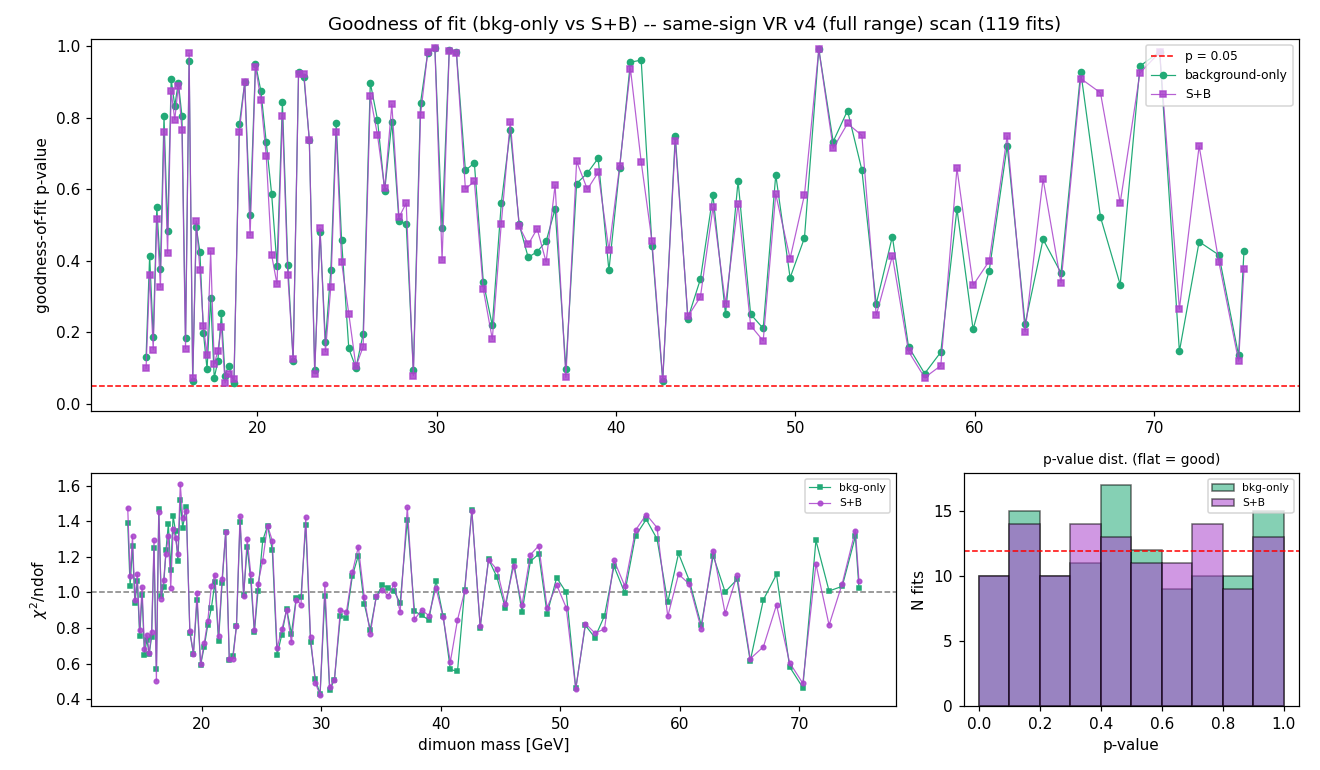
\includegraphics[width=0.95\linewidth]{Figures/6Control_Region_figures/Fitting/scan_bkg_gof.png}
    \caption{Goodness of fit over the 119 mass hypotheses of the same-sign control region scan.
    Top: the signal plus background and background-only goodness-of-fit $p$-value as a function of the di-muon mass hypothesis, with the $p = 0.05$ threshold indicated.
    Bottom left: the corresponding $\chi^2/\mathrm{ndof}$.
    Bottom right: the distribution of the $p$-values, which is consistent with the uniform distribution expected for an adequate background model.}
    \label{fig:cr_bkg_gof}
\end{figure}

The background functional form and fit window chosen by the adaptive procedure are summarized in Fig.~\ref{fig:cr_fit_config}.
The number of free background parameters selected by the F-test is low across the entire scan: a single parameter suffices for 75 of the 119 fits, two for 33, three for 10, and four for the single remaining fit.
The polynomial-times-exponential and exponential-of-a-polynomial families account for essentially all of the selected forms, while the more flexible high-order forms are almost never preferred, consistent with the smoothly falling same-sign spectrum; the sole exception is a fourth-order polynomial-times-exponential at 70.3\GeV, whose fit is nonetheless of good quality ($p = 0.98$).
The adaptive window stays at its nominal $\pm 7\sigma$ for the large majority of fits, shrinking to between $\pm 4\sigma$ and $\pm 6.5\sigma$ at 8 of the 119 mass hypotheses, where the nominal window gives a poor goodness of fit.

\begin{figure}[!h]
    \centering
    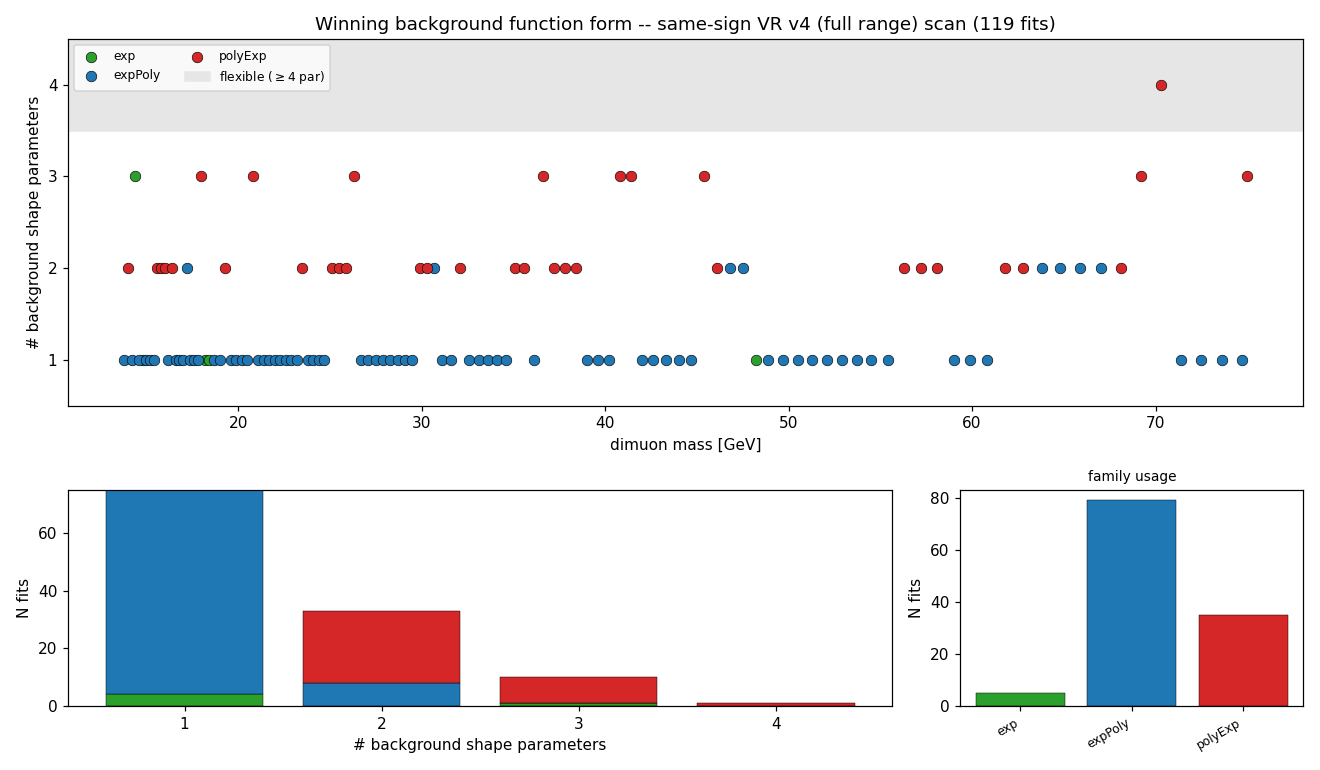
\includegraphics[width=0.49\linewidth]{Figures/6Control_Region_figures/Fitting/scan_func_forms.png}
    \hfill
    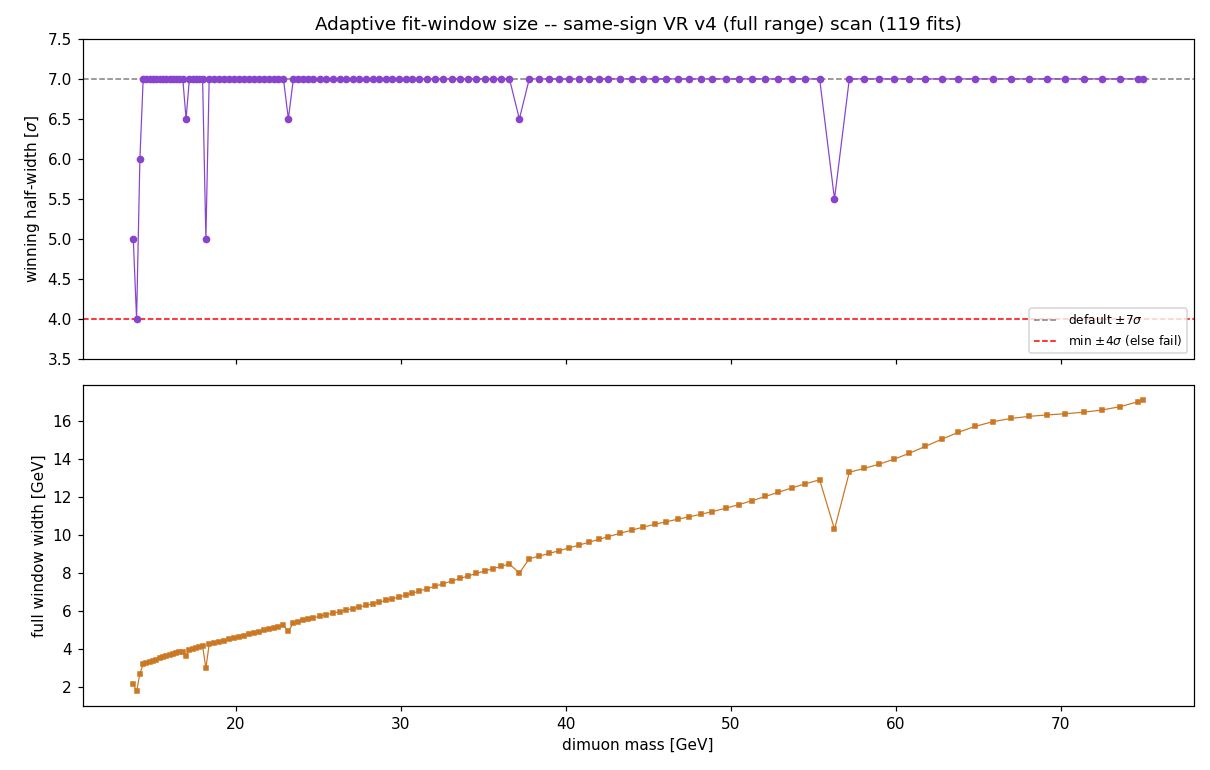
\includegraphics[width=0.49\linewidth]{Figures/6Control_Region_figures/Fitting/scan_window_sizes.png}
    \caption{Fit configuration selected by the adaptive procedure across the 119 mass hypotheses of the same-sign control region scan.
    Left: the winning background functional form as a function of the di-muon mass hypothesis, coloured by family, with the number of free background parameters on the vertical axis; the lower panels show the distribution of the number of parameters and the overall usage of each family.
    Right: the winning fit-window half-width in units of the local resolution $\sigma$ (top), which remains at the nominal $\pm 7\sigma$ apart from a few adaptively shrunk points, and the corresponding full window width in \GeVns\ (bottom).}
    \label{fig:cr_fit_config}
\end{figure}

The sensitivity of the scan to a localized signal is quantified by the local significance of the fitted signal yield at each mass hypothesis, shown in Fig.~\ref{fig:cr_significance}.
The significances scatter symmetrically about zero and lie between $-2.2\sigma$ and $+2.6\sigma$ across the search range.
The largest local significance is $+2.6\sigma$, at a mass hypothesis of 67.0\GeV.
Given the 119 correlated hypotheses tested, a local fluctuation of this size is fully consistent with the background-only expectation, and no globally significant excess is present.
An example fit, at this most significant mass hypothesis, is shown in Fig.~\ref{fig:cr_postfit_example}; even here the fit is of good quality ($p = 0.87$) and the corresponding excess of $26 \pm 9$ signal events is not significant.

\begin{figure}[!h]
    \centering
    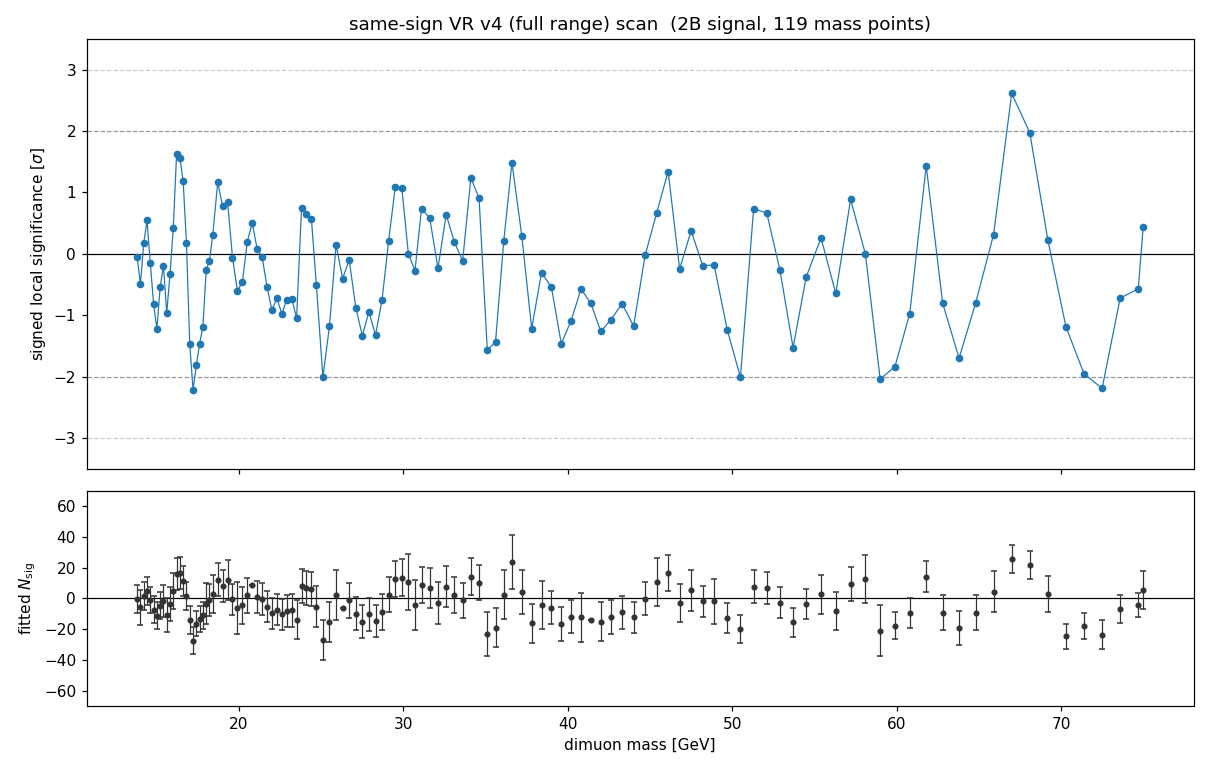
\includegraphics[width=0.95\linewidth]{Figures/6Control_Region_figures/Fitting/scan_significance.png}
    \caption{Signed local significance of the fitted signal yield (top) and the fitted signal yield $N_\mathrm{sig}$ with its uncertainty (bottom) as a function of the di-muon mass hypothesis, for the 119 fits of the same-sign control region scan.
    The significances scatter symmetrically about zero and lie within $\pm 2.6\sigma$ over the full range, with the largest excursion, $+2.6\sigma$, at 67.0\GeV.}
    \label{fig:cr_significance}
\end{figure}

\begin{figure}[!h]
    \centering
    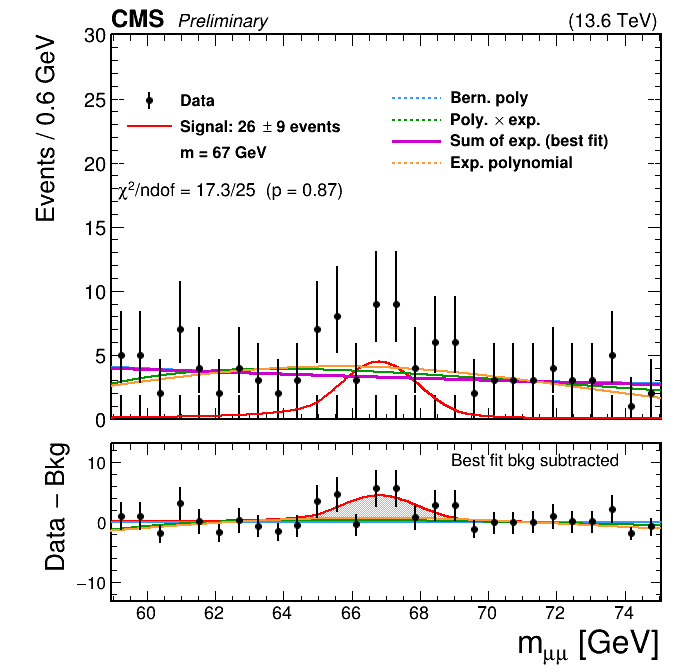
\includegraphics[width=0.6\linewidth]{Figures/6Control_Region_figures/Fitting/cr_postfit_example.png}
    \caption{Example signal-plus-background fit in the same-sign control region, at the most significant mass hypothesis of the scan (67.0\GeV).
    Data (black points) are compared to the best-fit signal-plus-background model, the background component of the selected functional form, and the fitted signal contribution.
    The lower panel shows the residual after subtracting the best-fit background.
    Even at the largest local fluctuation of the scan the fit is of good quality ($p = 0.87$) and the corresponding excess of $26 \pm 9$ signal events is not significant.}
    \label{fig:cr_postfit_example}
\end{figure}

A representative selection of nine signal-plus-background fits, spanning the search range from 14 to 72\GeV, is shown in Fig.~\ref{fig:cr_postfit_grid}.
Across this range the background model describes the data well, the fitted signal yield is consistent with zero, and the residuals show no coherent peaking structure, illustrating that the good fit quality summarized above holds uniformly across the scan.

\begin{figure}[!h]
    \centering
    %--- Row 1 ---
    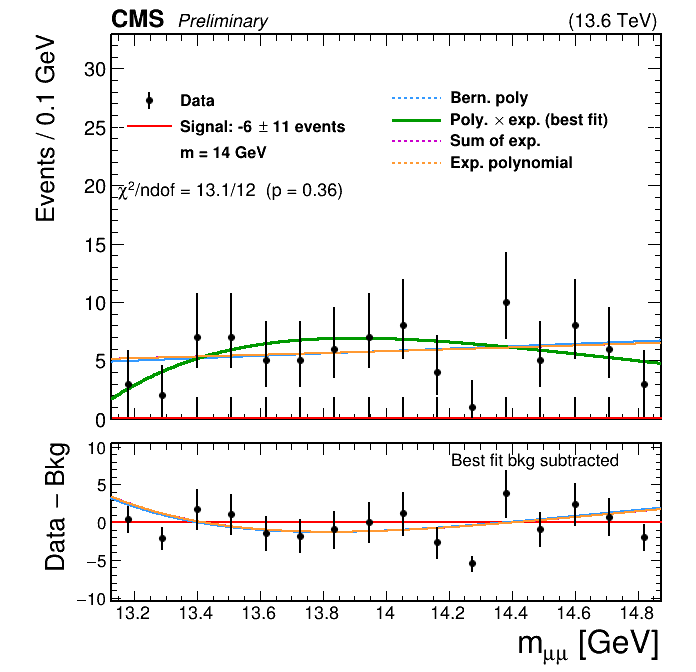
\includegraphics[width=0.32\linewidth]{Figures/6Control_Region_figures/Fitting/cr_postfit_M14.png}
    \hfill
    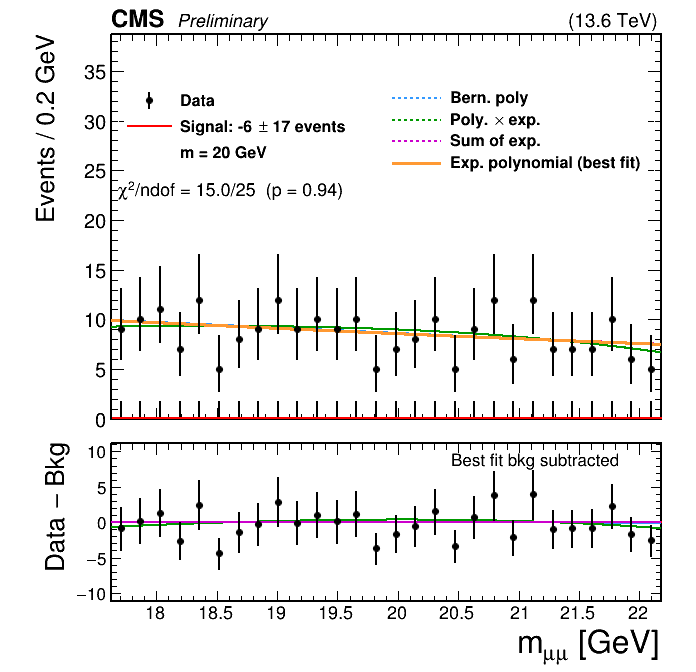
\includegraphics[width=0.32\linewidth]{Figures/6Control_Region_figures/Fitting/cr_postfit_M20.png}
    \hfill
    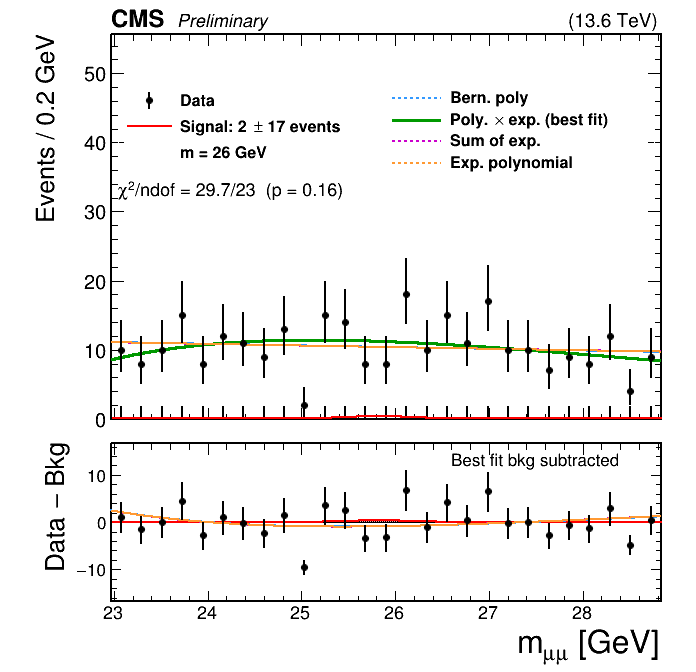
\includegraphics[width=0.32\linewidth]{Figures/6Control_Region_figures/Fitting/cr_postfit_M26.png}

    \vspace{0.5em}

    %--- Row 2 ---
    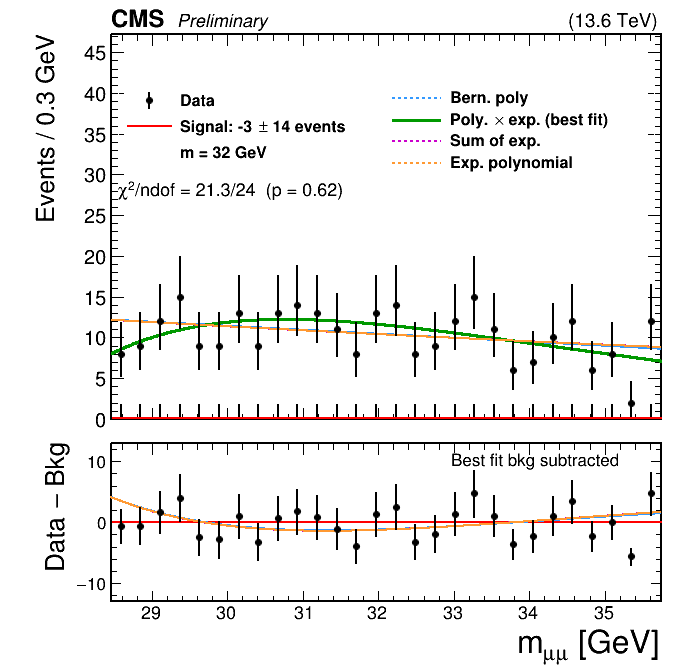
\includegraphics[width=0.32\linewidth]{Figures/6Control_Region_figures/Fitting/cr_postfit_M32.png}
    \hfill
    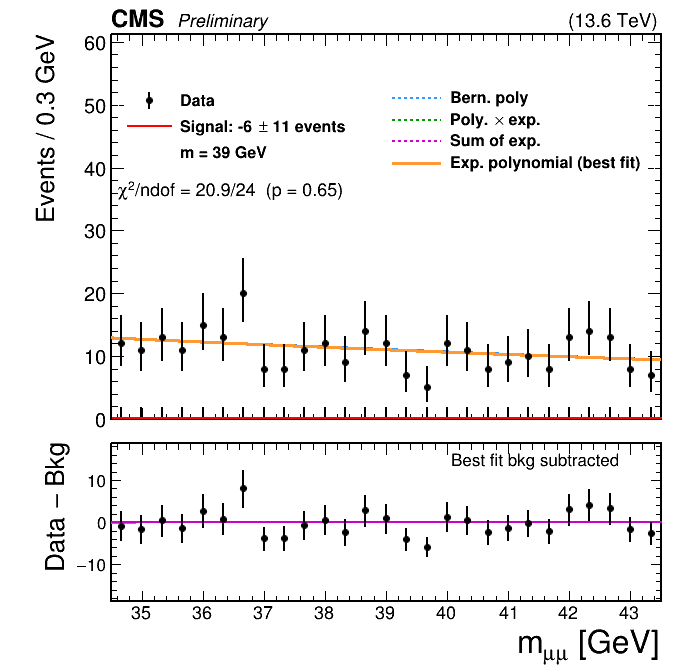
\includegraphics[width=0.32\linewidth]{Figures/6Control_Region_figures/Fitting/cr_postfit_M39.png}
    \hfill
    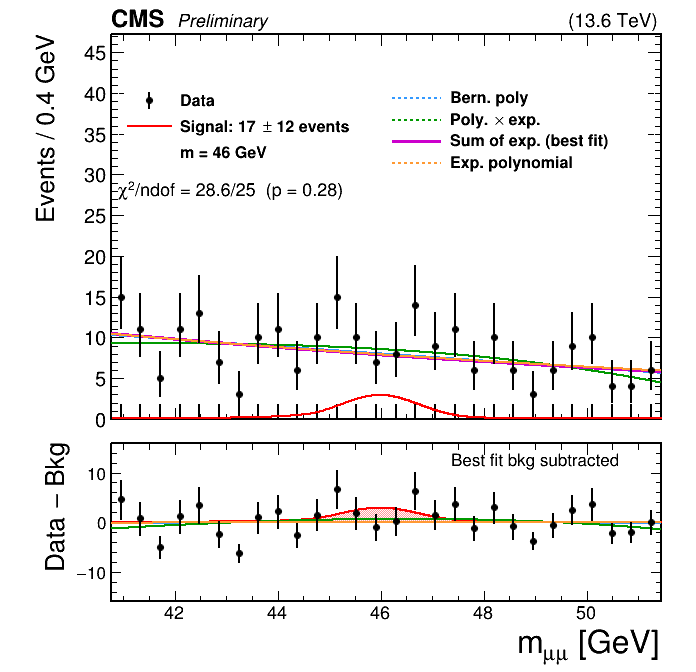
\includegraphics[width=0.32\linewidth]{Figures/6Control_Region_figures/Fitting/cr_postfit_M46.png}

    \vspace{0.5em}

    %--- Row 3 ---
    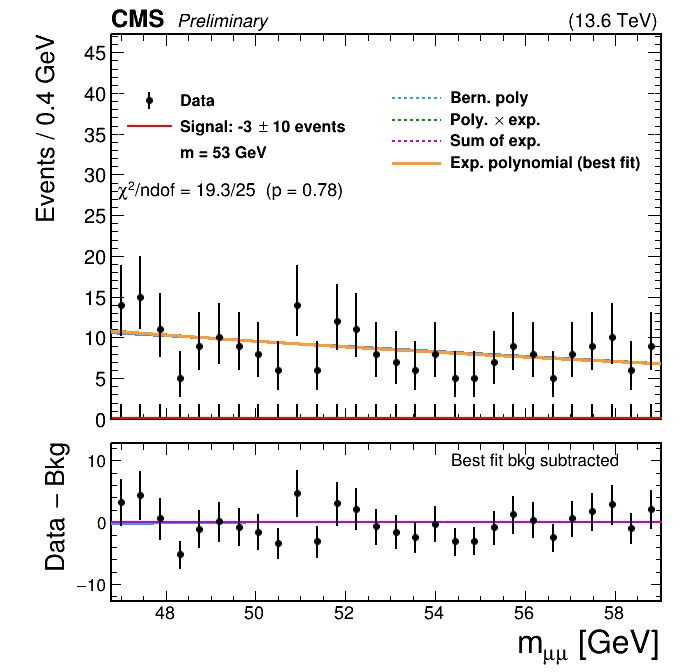
\includegraphics[width=0.32\linewidth]{Figures/6Control_Region_figures/Fitting/cr_postfit_M53.png}
    \hfill
    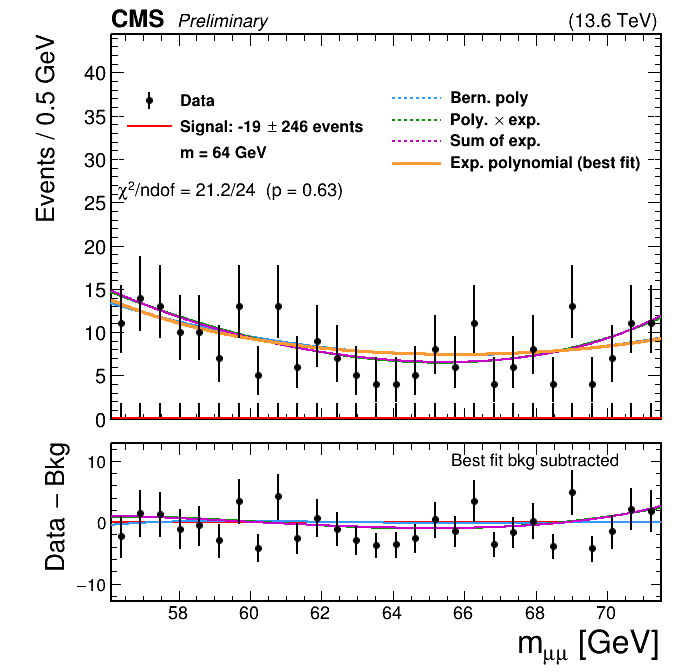
\includegraphics[width=0.32\linewidth]{Figures/6Control_Region_figures/Fitting/cr_postfit_M64.png}
    \hfill
    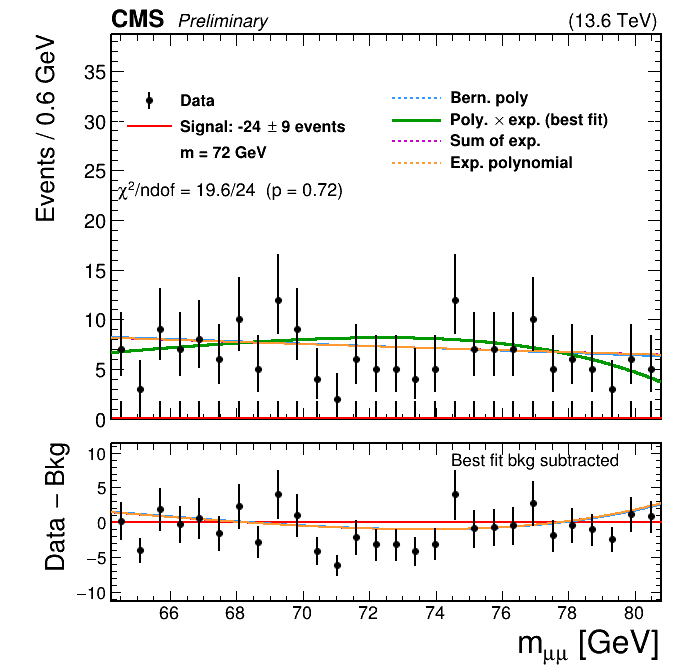
\includegraphics[width=0.32\linewidth]{Figures/6Control_Region_figures/Fitting/cr_postfit_M72.png}

    \caption{Representative signal-plus-background fits in the same-sign control region at nine mass hypotheses spanning the search range (approximately 14, 20, 26, 32, 39, 46, 53, 64 and 72\GeV).
    In each panel the data (black points) are compared to the best-fit signal-plus-background model, the background component of the selected functional form, and the fitted signal contribution, with the $\chi^2/\mathrm{ndof}$ and background-only $p$-value indicated.
    The lower panel of each plot shows the residual after subtracting the best-fit background.
    The fitted signal is consistent with zero at all masses and no localized excess is present, confirming that the CATHODE pipeline does not sculpt the $m_{\mu\mu}$ spectrum.}
    \label{fig:cr_postfit_grid}
\end{figure}

The absence of any significant excess across the full set of mass hypotheses validates the CATHODE pipeline for use in the opposite-sign signal region: the generative model, classifier, and fit procedure do not introduce artificial structure in the $m_{\mu\mu}$ spectrum when no signal is present.

\fi % end \ifboth